\chapter{Basic math routines}
\begin{refsection}

\abstract{\texttt{MathFunc} contains basic math functions beyond the routines already available in the Lazarus-library \texttt{math}. It also defines important mathematical and natural constants and the typed constants (changeable by the user program) \texttt{ValidFigures, MaxError, MaxIter, Zero}.}

The interface is:

\begin{lstlisting}[caption=Interface of unit MathFunc]
  UNIT MathFunc;

  INTERFACE

  USES Math;
  // IN Lazarus no need to reinvent the wheel, otherwise uncomment important routines at the end

  CONST
    MathError: BOOLEAN = FALSE;   // toggle FOR error condition
    PowerOfTwo: ARRAY[0..30] OF LONGINT =
      (       1,         2,          4,          8,         16,         32,
             64,       128,        256,        512,       1024,       2048,
           4096,      8192,      16384,      32768,      65536,     131072,
         262144,    524288,    1048526,    2097152,    4194304,    8388608,
       16777216,  33554432,   67108864,  134217728,  268435456,  536870912,
     1073741824);

  TYPE
    ByteStr = STRING[2];
    float   = double;                    // allows global switch of precission

  CONST
    ValidFigures: BYTE  = 10;            // Ziffern bei der Ausgabe
    MaxError    : float = 1e-7;          // Konvergenz-Kriterium
    MaxIter     : WORD  = 1000;          // falls keine Konvergenz
    Zero        : float = 1e-100;        // kleinste Number <> 0

    MachineEpsilon = 2.2204460492503130E-16;   // Maschinen-abhängig
    MaxRealNumber  = 1.7976931348623150E+308;
    MinRealNumber  = 2.2250738585072020E-308;

    Const_pi    = 3.141592653589793238462643383280;  // Kreiszahl
    Const_2pi   = 2 * Const_pi;
    Const_e     = 2.718281828459045235360287471353;  // Euler'sche Zahl
    Const_ln2   = 0.693147180559945309417232121458;  // nat. log. von 2
    Const_ln10  = 2.302585092994045684017991454684;  // nat. log. von 10
    Const_delta = 4.669201609102990671853203820466;  // Feigenbaum-Konstante
    Const_phi   = (1 + sqrt(5)) / 2;                 // goldener Schnitt
    Const_Sqrt2 = sqrt(2);


    Const_a0    = 5.29177210903e-11;             // Bohr-radius, radius of H atom, m
    Const_alpha = 7.2973525693e-3;               // Finestructure (Sommerfeld) constant
    Const_g     = 9.80665;                       // Fallbeschleunigung Erde, m/s^2
    Const_Gamma = 6.67430e-11;                   // Gravitationskonstante, N m^2 / kg^2
    Const_Na    = 6.0221367e23;                  // Avogadro-Konstante, mol^-1
    Const_kB    = 1.380658e-23;                  // Boltzmann-Konstante, J/K
    Const_F     = 96485.33289;                   // Faraday-Konstante, J / (mol V) = C/mol
    Const_c     = 299792458;                     // Lichtgeschwindigkeit, m/s
    Const_h     = 6.6260755e-34;                 // Plank'sches Wirkungsquantum, J s
    Const_bar_h = Const_h / Const_2pi;
    Const_me    = 9.10938356e-31;                // Elektronenmasse, kg
    Const_mp    = 1.672621898e-27;               // Protonmasse, kg
    Const_mn    = 1.674927471e-27;               // Neutronenmasse, kg
    Const_Ce    = 1.60217733e-19;                // Elementarladung, A s
    Const_R     = 8.3144598;                     // Gaskonstante, J / (mol kg)
    Const_e0    = 8.854187817e-12;
    // elektrische Feldkonstante, A^2 s^4 / (kg m^3) = C / (V m)
    Const_m0    = 1.2566e-6;
    // magnetische Feldkonstante, kg m / (A^2 s^2) = N / A^2
    Const_vCs   = 9192631770;                    // Freq 133-Cs, Hz
    Const_Km    = 683;                           // Strahlungsausbeute 540 THz (5550 nm), lm/W

  FUNCTION FloatStr(Number: float; ValidFigures: BYTE): STRING;
  { create a string from real number, having defined length. Minimum length is 8 }

  FUNCTION ReadFloat(VAR Medium: TEXT): float;

  FUNCTION ReadInt(VAR Medium: TEXT): LONGINT;

  FUNCTION RoundTo(Number: float; RoundAfter: float): float;
  { Bsp: RoundTo(5.4321, 0.01) = 5.43 }

  FUNCTION WriteErrorMessage(TEXT: STRING): CHAR;

  FUNCTION Signum(x: float): INTEGER;
  { +1 for x > 0, -1 for x < 0 and 0 for x=0 }

  FUNCTION Max(a, b: float): float;
  { Maximal Value of two numbers  }

  FUNCTION Max(a, b: LONGINT): LONGINT;

  FUNCTION Min(a, b: float): float;
  { minimal value of two numbers  }

  FUNCTION Min(a, b: LONGINT): LONGINT;

  FUNCTION Pythag(a, b: float): float;
  { computes sqrt(sqr(a) + sqr(b)) without over/undeflow }

  FUNCTION GCD(n1, n2: LONGINT): LONGINT;
  { greatest common denominator }

  FUNCTION SCM(n1, n2: LONGINT): LONGINT;
  { smallest common multiple }

  FUNCTION DecimalFraction(a: float; VAR Zaehler, Nenner: WORD): BOOLEAN;
  { Umwandlung eines Dezimalbruches a in Fraction aus ganzen Zahlen. Funktion wird
    true, wenn abs(a - Zaehler / Nenner) < MaxError }

  FUNCTION Pot(Basis: float; Exponent: LONGINT): float;
  { Potenzfunktion mit ganzzahligem Exponenten }

  FUNCTION Pot(Basis, Exponent: float): float;
  { Potenz-Funktion, Basis und Exponent reel }

  FUNCTION log(x, Basis: float): float;
  { Allgemeine log Funktion mit beliebiger Basis }

  FUNCTION xCoordinate(x1, y1, x2, y2, x3, y3, x4, y4: float): float;
  { x-coordinate of intersection between lines (x1, y1), (x2, y2) and
    (x3, y3), (x4, y4) }

  FUNCTION yCoordinate(x1, y1, x2, y2, x3, y3, x4, y4: float): float;
  { y-coordinate of intersection }

  {************************** Winkel-Funktionen ****************************}

  FUNCTION Grad(x: float): float;
  {Radiant nach Grad}

  FUNCTION Rad(x: float): float;
  { Grad nach Radiant }

  FUNCTION coth(x: float): float;
  { cotangens hyperbolicus }

  FUNCTION sech(x: float): float;
  { secans hyperbolicus }

  FUNCTION csch(x: float): float;
  { cosecans hyperbolicus }

  FUNCTION ArCoth(x: float): float;
  { area cotangens hyperbolicus }

  FUNCTION ArSech(x: float): float;
  { area secans hyperbolicus }

  FUNCTION ArCsch(x: float): float;
  { area cosecans hyperbolicus }

  FUNCTION Sec(x: float): float;
  { Secans }

  FUNCTION Csc(x: float): float;
  { Cosecans }

  FUNCTION ArcCot(x: float): float;
  {arcus cotangens}

  FUNCTION ArcSec(x: float): float;
  {Arcus Secans}

  FUNCTION ArcCsc(x: float): float;
  { Arcus Cosecans }

  {****************** Funktionen für Statistik ****************************}

  FUNCTION LnGamma(x: float): float;
  { Logarithmus der Gamma-Funktion }

  FUNCTION fak(i: BYTE): LONGINT;

  FUNCTION LnFak(x: float): float;
  { Log(x!) calculated via gamma-function }

  FUNCTION IncompleteGamma(a, x: float): float;
  { Numerical Recipes p. 182 }

  FUNCTION BinomialCoef(n, k: LONGINT): float;
  { Binominal-Koeffizient, Anzahl der Möglichkeiten, k Elemente aus n auszuwählen }

  { *********************** Diverses ***************************** }

  FUNCTION HexByte(Number: BYTE): ByteStr;
  { Umwandlung einer Number von Dezimal nach Hexadezimal }

  FUNCTION InWorten(Number: LONGINT): STRING;
  { Wandelt eine Number in Worte um (für Finanzmathematik). Es muß gelten:
    abs(Number) < 1.000.000 }

  FUNCTION Modulo11(Number: LONGINT): CHAR;
  { gibt den Prüfcode nach dem modulo-11 Verfahren zurück(eine Ziffer von 0..9
    oder den Buchstaben "X") \parencite{Mic-96}.

  FUNCTION TestModulo11(Number: LONGINT; TEST: CHAR): BOOLEAN;
  { Testet ob eine Number zu ihrer Prüfziffer paßt }


  IMPLEMENTATION

  VAR
    CH: CHAR;
\end{lstlisting}

\section{Administrative functions}

The routines of this unit can pass error conditions to the calling program by setting an error flag \texttt{MathError}. In addition, an error message is produced:
\begin{lstlisting}[caption=Error handling]
FUNCTION WriteErrorMessage(Text: STRING): CHAR;

BEGIN
  Write(Text);
  ReadLn(Result);
END;
\end{lstlisting}
The calling program can then try to correct the error and then reset the error flag, or it can gracefully abort. User input is passed on as single character, the error message could contain a question \Foreign{a la}: ``Abort, ignore, continue?''  All units described here use this mechanism.

Conversion of a number \(x \in \mathbb{R} \) into a string for output is straight forward. The number of decimal places can be set, \acs{NaN} is handled:
\begin{lstlisting}[caption=Conversion of floating point number to string]
  FUNCTION FloatStr(Number: float; ValidFigures: BYTE): STRING;

  VAR
    hst: STRING;
    i: BYTE;

  BEGIN
    IF IsNaN(Number)
      THEN
        BEGIN
          hst := ' ';
          FOR i := 1 TO (ValidFigures - 3) DO
            hst := hst + ' ';
          Result := hst + 'NaN';
          EXIT;
        END;
    IF Abs(Number) < Zero
      THEN Number := 0.0;
    Str(Number: ValidFigures, hst);
    Result := hst;
  END;
\end{lstlisting}

The following routine reads a whole number (anything assignment compatible with longint) from a file. Characters that separate numbers are in the set \texttt{SepChar}.

\begin{lstlisting}[caption=Read whole numbers from file]
  FUNCTION ReadInt(VAR Medium: TEXT): LONGINT;

  CONST
    SepChar: SET OF CHAR = [';', ' '];   // separator between numbers
    NumChar: SET OF CHAR = ['0'..'9', '-'];

  VAR
    s: STRING;
    x: float;
    Error: INTEGER;

  BEGIN
    s := '';
    REPEAT
      Read(Medium, c);
      IF (c IN NumChar)
        THEN s := s + c;
    UNTIL (c IN SepChar) OR EoLn(Medium);
    Val(s, x, Error);
    IF Error <> 0
      THEN
        BEGIN
          ch := WriteErrorMessage('"' + s + '" is not a number');
          MathError := TRUE;
          EXIT;
        END;
    Result := Round(x);
  END;
\end{lstlisting}

Reading floating point numbers works in the same way, however, there are additional complications:
\begin{itemize}
  \item{we need to handle \acs{NaN} (expressed as 'NA' or 'NaN')}
  \item{we need to handle numbers written as potency of 10}
  \item{in different countries, different characters are used as decimal separator}
  \item{this implies different number separators in .csv-files}
\end{itemize}

\begin{lstlisting}[caption=Read floating point number from file]
  FUNCTION ReadFloat(VAR Medium: TEXT): float;

  CONST
    SepChar: SET OF CHAR = [';'];        // separator between numbers
    NumChar: SET OF CHAR = ['0'..'9', '-', '+', 'E', 'e', 'N', 'A', 'n', 'a'];
    DecSep = [',', '.'];   // decimal separator

  VAR
    s: STRING;
    x: float;
    Error: INTEGER;

  BEGIN
    s := '';
    REPEAT
      Read(Medium, c);
      IF (c IN DecSep)
        THEN s := s + '.'
        ELSE IF (c IN NumChar)
               THEN s := s + c
               ELSE IF (c IN SepChar) OR (c = ' ')
                      THEN // DO nothing
                      ELSE // illegal character
                        BEGIN
                          s := s + c;
                          ch := WriteErrorMessage(s + ' is not a number');
                          MathError := TRUE;
                          EXIT;
                        END;
    UNTIL (c IN SepChar) OR EoLn(Medium);
    IF ((UpCase(s) = 'NA') OR (UpCase(s) = 'NAN'))
      THEN
        BEGIN
          ReadFloat := NaN;
          EXIT;
        END;
    Val(s, x, Error);
    IF Error <> 0
      THEN
        BEGIN
          ch := WriteErrorMessage(s + ' is not a number');
          MathError := TRUE;
          EXIT;
        END;
    Result := x;
  END;
\end{lstlisting}

Rounding is accomplished to a given precision:
\begin{lstlisting}[caption=]
  FUNCTION RoundTo(Number: float; RoundAfter: float): float;

  BEGIN
    Result := RoundAfter * Int(Number / RoundAfter + 0.5);
  END;
\end{lstlisting}
For example, \texttt{Round(5.4321, 0.01)} results in \num{5.43}.

The signum function returns \(\pm 1 \) depending on the sign of \skalar{x}, or \num{0} if \skalar{x} is very small:
\begin{lstlisting}[caption=Signum function]
  FUNCTION Signum(x: float): INTEGER;

  BEGIN
    IF (x < -Zero)
      THEN Result := -1
      ELSE IF (x > Zero)
             THEN Result := 1
             ELSE Result := 0;
  END;
\end{lstlisting}
``Very small'' is defined by the typed constant \texttt{Zero}, which can be adjusted by the calling program according to needs.

\section{Integer arithmetic}

The following routines calculate the largest common denominator, the smallest common multiple and convert a decimal number into a fraction or a Hex-string:
\begin{lstlisting}[caption=Integer arithmetic]
  FUNCTION GCD(n1, n2: LONGINT): LONGINT;

  VAR
    r: LONGINT;

  BEGIN
    IF n2 <> 0
      THEN
        BEGIN
          REPEAT
            r := n1 MOD n2;
            n1 := n2;
            n2 := r;
          UNTIL r = 0;
          Result := n1;
        END
      ELSE
        IF n1 = 0
          THEN
            Result := 0         { GCD(0,0) = 0 }
          ELSE
            BEGIN
              WriteErrorMessage('division by 0');
              MathError := TRUE;
              EXIT;
            END;
  END;


  FUNCTION SCM(n1, n2: LONGINT): LONGINT;

  VAR
    n: LONGINT;

  BEGIN
    n := GCD(n1, n2);
    IF n <> 0
      THEN Result := n1 * n2 DIV GCD(n1, n2)
      ELSE Result := 0;
  END;


  FUNCTION DecimalFraction(a: float; VAR Zaehler, Nenner: WORD): BOOLEAN;

  VAR
    temp1, temp2, Teil1, Teil2: float;
    Iter, Num: WORD;

  BEGIN
    iter := 0;
    Temp1 := a;
    Teil1 := 0.0;
    Teil2 := 1.0;
    Zaehler := 1;
    Nenner := 0;
    REPEAT
      INC(Iter);
      Num := Trunc(Temp1);
      temp2 := Zaehler;
      Zaehler := Round(Num * Zaehler + Teil1);
      Teil1 := Temp2;
      Temp2 := Nenner;
      Nenner := Round(Num * Nenner + Teil2);
      Teil2 := Temp2;
      Temp1 := 1 / (Temp1 - Num);
    UNTIL (iter > MaxIter) OR (Abs(a - Zaehler / Nenner) < MaxError);
    Result := Iter <= MaxIter;
  END;


  FUNCTION HexByte(Number: BYTE): ByteStr;

  CONST
    Ziffern: ARRAY [0..15] OF CHAR = '0123456789ABCDEF';

  BEGIN
    HexByte[1] := Ziffern[Number SHR 4];
    HexByte[2] := Ziffern[Number AND $0F];
  END;
\end{lstlisting}

\section{Maximum and minimum of two numbers}

Here we use overloading so that both integer and real variables can be used:

\begin{lstlisting}[caption=Maximum and minimum]
  FUNCTION Max(a, b: float): float;

  BEGIN
    IF (a > b)
      THEN Result := a
      ELSE Result := b;
  END;

  FUNCTION Min(a, b: float): float;

  BEGIN
    IF (a < b)
      THEN Result := a
      ELSE Result := b;
  END;


  FUNCTION Max(a, b: LONGINT): LONGINT;

  BEGIN
    IF (a > b)
      THEN Result := a
      ELSE Result := b;
  END;

  FUNCTION Min(a, b: LONGINT): LONGINT;

  BEGIN
    IF (a < b)
      THEN Result := a
      ELSE Result := b;
  END;
\end{lstlisting}


\section{Exponents, logarithms, powers}

\( f(x,y) = x^y \) is defined in different ways depending on whether \(x, y \in \mathbb{R} \) or \(\in \mathbb{N} \):
\begin{description}
  \item[ \( y = 0 \)]{\(z = x^0 = 1 \).}
  \item[ \( x = 0 \)]{\(z = 0^y = 0 \), except for \(y=0 \).}
  \item[ \( y \in \mathbb{N} \)]{\hspace{10mm}
    \begin{description}
       \item[\( y > 0 \)]{\( z = x \times x \times \ldots \times x \), \skalar{y} times.}
       \item[\(y < 0 \)]{ \(z = 1/x \times 1/x \times \ldots \times 1/x \), \skalar{-y} times.}
    \end{description}}
  \item[\(y \in \mathbb{R} \)]{\hspace{10mm}
    \begin{description}
       \item[\(x > 0 \)]{\(z = \exp(\ln(x) * y) \).}
       \item[\(x < 0 \)]{\skalar{z} undefined, raise error condition.}
    \end{description}}
\end{description}
This is easiest done by overloading the function for the case exponent \( \in \mathbb{N} \) or \( \in \mathbb{R} \):

\begin{lstlisting}[caption=Universal power function]
  FUNCTION Pot(Basis: float; Exponent: LONGINT): float;

  VAR
    Product: float;
    i: LONGINT;

  BEGIN
    IF Exponent = 0
      THEN
        BEGIN
          Result := 1;
          EXIT;
        END;
    IF Abs(Basis) < Zero
      THEN
        BEGIN
          Result := 0;
          EXIT;
        END;
    IF Exponent < 0
      THEN
        BEGIN
          Basis := 1 / Basis;
          Exponent := -Exponent;
        END;
    Product := 1;
    FOR i := 1 TO Exponent DO
      Product := Product * Basis;
    Result := Product;
  END;

  FUNCTION Pot(Basis, Exponent: float): float;

  BEGIN
    IF Abs(Exponent) < Zero
      THEN
        BEGIN
          Result := 1;
          EXIT;
        END;
    IF Abs(Basis) < Zero
      THEN
        BEGIN
          Result := 0;
          EXIT;
        END;
    IF Basis > Zero     // Basis > 0
      THEN
        Result := Exp(Ln(Basis) * Exponent)
      ELSE
        BEGIN
          CH := WriteErrorMessage('Power negative base and real exponent');
          Matherror := TRUE;
        END;
  END;
\end{lstlisting}


\begin{lstlisting}[caption=Universal log]
  FUNCTION log(x, Basis: float): float;

  BEGIN
    IF x > Zero
      THEN
        Result := Ln(x) / Ln(Basis)
      ELSE
        BEGIN
          CH := WriteErrorMessage('log(x) mit x < 0');
          EXIT;
        END;
  END;
\end{lstlisting}

\begin{lstlisting}[caption=Pytagoras]
  FUNCTION Pythag(a, b: float): float;

  VAR
    at, bt: float;

  BEGIN
    at := Abs(a);
    bt := Abs(b);
    IF (at > bt)
      THEN
        Result := at * Sqrt(1.0 + Sqr(bt / at))
      ELSE
        IF (bt = 0)
          THEN Result := 0
          ELSE Result := bt * Sqrt(1.0 + Sqr(at / bt));
  END;
\end{lstlisting}

\section{Intersection of two lines }

If we have two lines, given by two points each, we can calculate the coordinates of their intersection. This is for example used for the ``direct plot'' of \Name{Eisenthal \& Cornish-Bowden} \parencite{Cor-74,Eis-74}.

\begin{lstlisting}[caption=Intersection of lines]
  FUNCTION xCoordinate(x1, y1, x2, y2, x3, y3, x4, y4: float): float;
    // x-coordinate OF intersection OF between lines given by 2 points each

  BEGIN
    Result := ((x1 * y2 - y1 * x2) * (x3 - x4) - (x1 - x2) * (x3 * y4 - y3 * x4)) /
      ((x1 - x2) * (y3 - y4) - (y1 - y2) * (x3 - x4));
  END;

  FUNCTION yCoordinate(x1, y1, x2, y2, x3, y3, x4, y4: float): float;

  BEGIN
    Result := ((x1 * y2 - y1 * x2) * (y3 - y4) - (y1 - y2) * (y3 * y4 - y3 * x4)) /
      ((x1 - x2) * (y3 - y4) - (y1 - y2) * (x3 - x4));
  END;
\end{lstlisting}


\section{Conversion of angles between rad and degrees}

\begin{lstlisting}[caption=]
  FUNCTION Grad(x: float): float;
    {Bogenmaß in Altgrad umrechnen}

  BEGIN
    Result := x * 180 / Pi;
  END;


  FUNCTION Rad(x: float): float;
    {Altgrad in Bogenmaß umrechnen}

  BEGIN
    Result := x * Pi / 180;
  END;
\end{lstlisting}

\section{Hyperbolic functions}


\begin{lstlisting}[caption=]
  FUNCTION coth(x: float): float;

  VAR
    z: float;

  BEGIN
    z := sinh(x);
    IF (z <> 0)
      THEN
        Result := cosh(x) / z
      ELSE
        BEGIN
          CH := WriteErrorMessage('coth with sinh(x) = 0');
          MathError := TRUE;
        END;
  END;


  FUNCTION Sech(x: float): float;

  BEGIN
    Result := Sqrt(1 - Sqr(tanh(x)));
  END;


  FUNCTION Csch(x: float): float;

  BEGIN
    Result := Sqrt(Sqr(coth(x)) - 1);
  END;
\end{lstlisting}

\section{Area functions}

\begin{lstlisting}[caption=]
  FUNCTION ArCoth(x: float): float;

  BEGIN
    IF Abs(x) > 1.0
      THEN
        ArCoth := 0.5 * Ln((x + 1) / (x - 1))
      ELSE
        BEGIN
          CH := WriteErrorMessage('arcoth(x) with x not from [-1..1]');
          MathError := TRUE;
        END;
  END;


  FUNCTION ArSech(x: float): float;

  VAR
    y: float;

  BEGIN
    y := 1 / x + Sqrt(1 / Sqr(x) - 1);
    Result := log10(y);
  END;


  FUNCTION ArCsch(x: float): float;

  VAR
    y: float;

  BEGIN
    y := 1 / x + Sqrt(1 / Sqr(x) + 1);
    Result := log10(y);
  END;
\end{lstlisting}

\section{Cyclometric functions}

\begin{figure}[t]
 \caption{\capstart Definition of the cyclometric functions.   }
 \label{fig:cyclo}
 \centering
 \subfloat{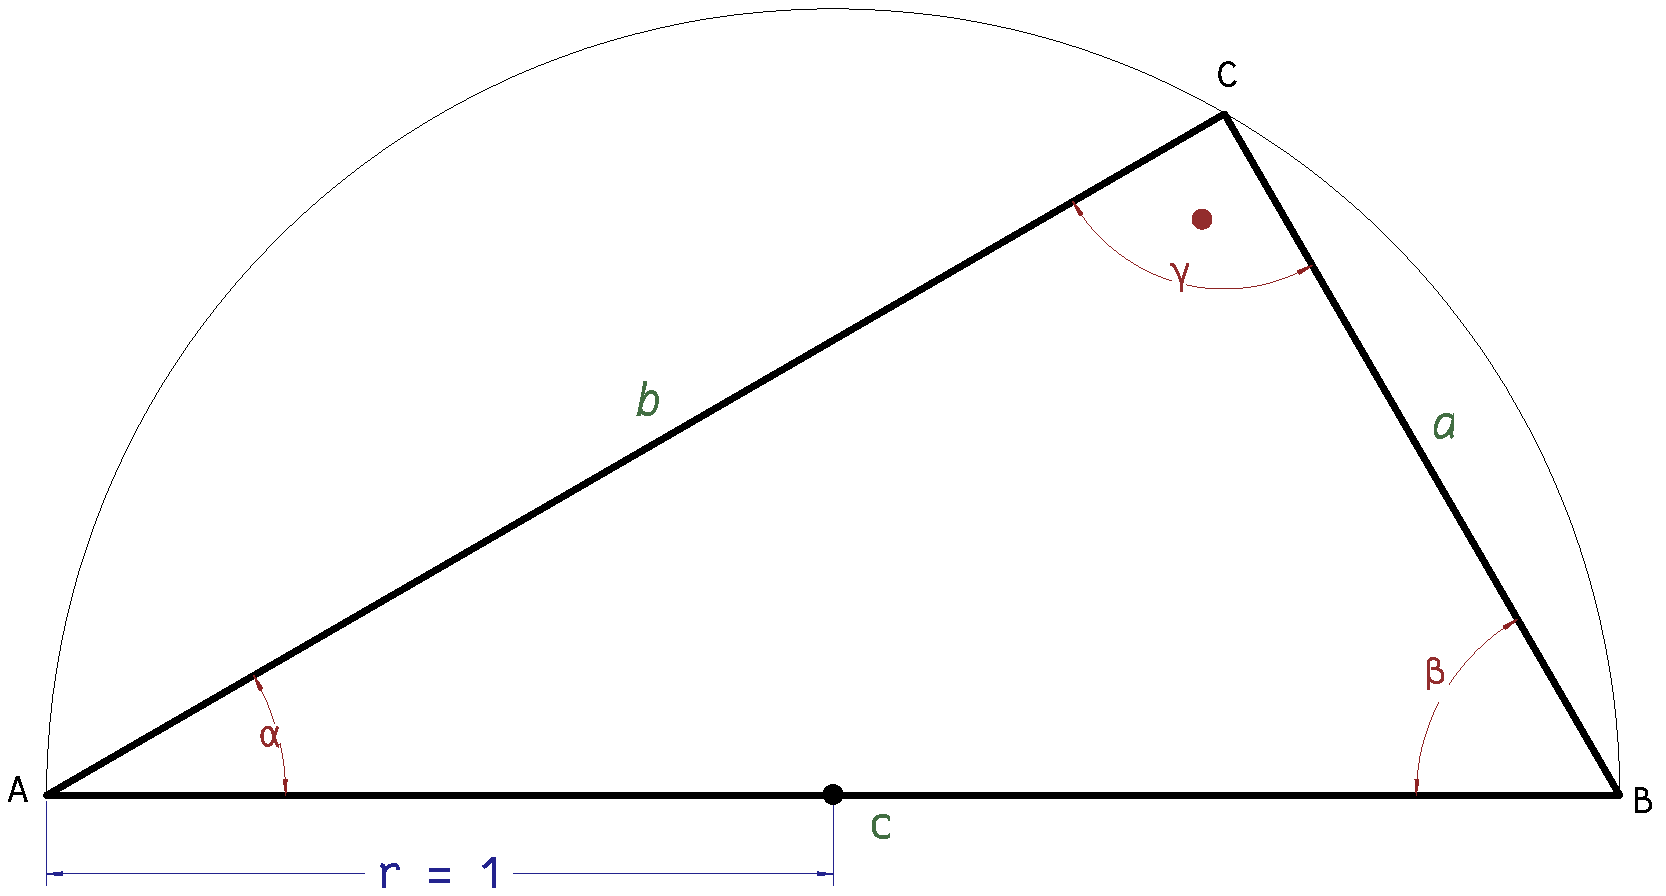
\includegraphics[width=0.5\textwidth]{Graphics/RightAngleTriangle}}\hfill
 \subfloat{\begin{tabular}{clc}
              \toprule
              Function              & Definition                            & Condition           \\
              \midrule
              sin(\skalar{\alpha})  & \skalar{a/c}                          & (\skalar{c \neq 0}) \\
              cos(\skalar{\alpha})  & \skalar{b/c}                          & (\skalar{c \neq 0}) \\
              tan(\skalar{\alpha})  & \skalar{a/b} = 1/cot(\skalar{\alpha}) & (\skalar{b \neq 0}) \\
              cot(\skalar{\alpha})  & \skalar{b/a} = 1/tan(\skalar{\alpha}) & (\skalar{a \neq 0}) \\
              sec(\skalar{\alpha})  & \skalar{c/b} = 1/cos(\skalar{\alpha}) & (\skalar{b \neq 0}) \\
              csc(\skalar{\alpha})  & \skalar{c/a} = 1/sin(\skalar{\alpha}) & (\skalar{a \neq 0}) \\
              \bottomrule
           \end{tabular} }
\end{figure}

For the sake of completeness, here some functions that are defined neither in standard Pascal, nor in the Lazarus \texttt{math} library:
\begin{lstlisting}[caption=Cyclometric functions]
  FUNCTION Sec(x: float): float;
    {Secans}

  VAR
    c: float;

  BEGIN
    c := Cos(x);
    IF c = 0
      THEN
        BEGIN
          CH := WriteErrorMessage('sec(x) with x = 90° or x = 270°');
          MathError := TRUE;
        END
      ELSE
        Result := 1 / c;
  END;


  FUNCTION Csc(x: float): float;

  VAR
    c: float;

  BEGIN
    c := Sin(x);
    IF c = 0
      THEN
        BEGIN
          CH := WriteErrorMessage('csc(x) with x = 90° or x = 270°');
          MathError := TRUE;
        END
      ELSE
        Result := 1 / c;
  END;

  FUNCTION ArcCot(x: float): float;

  BEGIN
    Result := Pi / 2 - ArcTan(x);
  END;


  FUNCTION ArcSec(x: float): float;

  BEGIN
    IF (x = 0) OR (Abs(x) > 1)
      THEN
        BEGIN
          CH := WriteErrorMessage('arcsec(x) with x not from [-1..1] or x = 0');
          MathError := TRUE;
        END
      ELSE
        Result := ArcCos(1 / x);
  END;


  FUNCTION ArcCsc(x: float): float;

  BEGIN
    IF (x = 0) OR (Abs(x) > 1)
      THEN
        BEGIN
          CH := WriteErrorMessage('arccsc(x) with x not from [-1..1] or x = 0');
          MathError := TRUE;
        END
      ELSE
        Result := ArcSin(1 / x);
  END;
\end{lstlisting}

\section{Routines required for statistics}

Even rather small numbers have large faculties, that can cause number overflows. The use of logarithms  avoids that problem:
\begin{lstlisting}[caption=logarithm of important functions]
  FUNCTION LnGamma(x: float): float;

  CONST
    a0 = 0.083333333096;
    a1 = -0.002777655457;
    a2 = 0.000777830670;
    c = 0.918938533205;

  VAR
    r: float;

  BEGIN
    r := (a0 + (a1 + a2 / Sqr(x)) / Sqr(x)) / x;
    Result := (x - 0.5) * Ln(x) - x + c + r;
  END;


  FUNCTION LnFak(x: float): float;

  VAR
    z: float;

  BEGIN
    z := x + 1;
    Result := LnGamma(z);
  END;
\end{lstlisting}

\begin{lstlisting}[caption=faculties (iterative)]
  FUNCTION fak(i: BYTE): LONGINT;

  VAR
    j: BYTE;
    Product: LONGINT;

  BEGIN
    Product := 1;    { fak(0) und fak(1) }
    FOR j := 2 TO i DO
      Product := Product * j;
    Result := Product;
  END;
\end{lstlisting}

The incomplete \( \gamma \)-function is calculated according to \parencite[p. 182]{Pre-89}, using either a series representation that converges quickly for \(x < a+1 \), or a continued fraction representation that converges quickly for \(x > a+1 \).

\subsection{Incomplete gamma-function}

\begin{lstlisting}[caption=Incomplete gamma function]
  FUNCTION IncompleteGamma(a, x: float): float;

  VAR
    GamSer, GamCF, gln: float;

    PROCEDURE GSer(a, x: float; VAR GamSer, gln: float);
    { series representation of incomplete gamma function, returns gamma in GamSer,
      ln(gamma) in gln. Converges quickly for x < succ(a) }

    VAR
      n: WORD;
      Sum, del, ap: float;

    BEGIN
      gln := LnGamma(a);
      IF (x <= 0)
        THEN
          BEGIN
            IF (x < 0)
              THEN
                BEGIN
                  ch := WriteErrorMessage('Error: Incomplete gamma-function: x < 0');
                  EXIT;
                END;
            GamSer := 0;
          END
        ELSE
          BEGIN
            ap := a;
            Sum := 1 / a;
            del := Sum;
            FOR n := 1 TO MaxIter DO
              BEGIN
                ap := ap + 1;
                del := del * x / ap;
                Sum := Sum + del;
                IF (Abs(del) < Abs(Sum) * MaxError)
                  THEN
                    BEGIN
                      ch := WriteErrorMessage(
                           'Error in incomplete gamma-function: no convergence ');
                      MathError := TRUE;
                      EXIT;
                    END;
              END;
            GamSer := Sum * Exp(-x + a * Ln(x) - gln);
          END;
    END;

    PROCEDURE gcf(a, x: float; VAR GamCF, gln: float);
    { continued fraction representation of incomplete gamma function, returns
      gamma in GamSer, ln(gamma) in gln. Converges quickly for x > succ(a) }

    VAR
      n: WORD;
      gOld, g, fac, b1, b0, anf, ana, an, a1, a0: float;

    BEGIN
      gln := LnGamma(a);
      gOld := 0.0;
      a0 := 1.0;
      a1 := x;
      b0 := 0.0;
      b1 := 1.0;
      fac := 1.0;
      FOR n := 1 TO MaxIter DO
        BEGIN
          an := 1.0 * n;
          ana := an - a;
          a0 := (a1 + a0 * ana) * fac;
          b0 := (b1 + b0 * ana) * fac;
          anf := an * fac;
          a1 := x * a0 + anf * a1;
          b1 := x * b0 + anf * b1;
          IF (a1 <> 0.0)
            THEN // renormalise
              BEGIN
                fac := 1.0 / a1;
                g := b1 * fac;
                IF (Abs((g - gOld) / g) < MaxError)
                  THEN  // convergence reached
                    BEGIN
                      GamCF := Exp(-x + a * Ln(x) - gln) * g;
                      EXIT;
                    END;
                gOld := g;
              END;
        END; // FOR
      ch := WriteErrorMessage('Error in incomplete gamma-function: no convergence');
      MathError := TRUE
    END;

  BEGIN
    IF (x < 0) OR (a <= 0)
      THEN
        BEGIN
          ch := WriteErrorMessage('Incomplete Gamma-function: arguments <= 0');
          MathError := TRUE;
          EXIT;
        END;
    IF (x < (a + 1.0))
      THEN
        BEGIN
          GSer(a, x, GamSer, gln);
          Result := 1.0 - GamSer;
        END
      ELSE
        BEGIN
          gcf(a, x, GamCF, gln);
          Result := GamCF;
        END;
  END;
\end{lstlisting}

\subsection{Binomial coefficients}

The binomial coefficient is the number of ways, in which \skalar{k} items can be chosen out of a set of \skalar{n}.
\begin{equation}
  \binom{n}{k} = \frac{n!}{k! (n-k)!} = \prod_{i=1}^k\frac{n + 1 -i}{i}
\end{equation}
The latter expression switches between multiplication and division, and hence avoids large numbers as much as possible. However, binomial coefficients -- even of relatively small numbers -- can be quite large, hence we use the float data type to avoid overflow.

\begin{lstlisting}[caption=binomial coefficient]
  FUNCTION BinomialCoef(n, k: LONGINT): float;

  VAR i,n1 : LONGINT;
    Res    : float;

  BEGIN
    IF n < k                // check FOR trivial cases first
      THEN Result := 0
      ELSE IF (n = k) OR (k = 0)
             THEN Result := 1
             ELSE IF k = 1
                    THEN Result := n
                    ELSE    // DO the real work
                      BEGIN
                        IF (2*k) > n THEN k := n-k;
                        Res := 1;
                        n1 := Succ(n);
                        FOR i := 1 TO k DO
                          Res := Res * (n1 - i) / i;
                        Result := Res;
                      END;
  END;
\end{lstlisting}


\section{Finance mathematics (with a German flavour)}

This routines converts a number into words

\begin{lstlisting}[caption=Finance mathematics]
  FUNCTION InWorten(Number: LONGINT): STRING;

  CONST
    Einer: ARRAY [1..9] OF STRING[6] =
      ('ein', 'zwei', 'drei', 'vier', 'fünf', 'sechs', 'sieben',
      'acht', 'neun');
    Zehner: ARRAY [1..9] OF STRING[8] =
      ('zehn', 'zwanzig', 'dreißig', 'vierzig', 'fünfzig',
      'sechzig', 'siebzig', 'achtzig', 'neunzig');
    Elfer: ARRAY [1..9] OF STRING[9] =
      ('elf', 'zwölf', 'dreizehn', 'vierzehn', 'fünfzehn', 'sechzehn',
      'siebzehn', 'achtzehn', 'neunzehn');

  VAR
    Minus: BOOLEAN;
    ZahlStr: STRING;
    ValueFeld: ARRAY [1..6] OF BYTE;

  BEGIN
    IF Number >= 1000000
      THEN
        BEGIN
          InWorten := ('Ungültiger Bereich ');
          EXIT;
        END;
    IF Number < 0
      THEN
        BEGIN
          Minus := TRUE;
          Number := Abs(Number);
        END
      ELSE
        Minus := FALSE;
    ValueFeld[1] := Number DIV 100000;    { Ziffern der Number isolieren }
    Number := Number MOD 100000;
    ValueFeld[2] := Number DIV 10000;
    Number := Number MOD 10000;
    ValueFeld[3] := Number DIV 1000;
    Number := Number MOD 1000;
    ValueFeld[4] := Number DIV 100;
    Number := Number MOD 100;
    ValueFeld[5] := Number DIV 10;
    ValueFeld[6] := Number MOD 10;
    ZahlStr := '';                     { String aufbauen, dabei die Besonderheiten }
    IF ValueFeld[1] > 0
      THEN ZahlStr := ZahlStr + Einer[ValueFeld[1]] + 'hundert';
    CASE ValueFeld[2] OF
      2..9: BEGIN
              IF ValueFeld[3] = 0
                THEN ZahlStr := ZahlStr + Zehner[ValueFeld[2]] + 'tausend'
                ELSE ZahlStr := ZahlStr + Einer[ValueFeld[3]] + 'und' +
                     Zehner[ValueFeld[2]] + 'tausend';
            END;
      1:    BEGIN
              IF ValueFeld[3] = 0
                THEN ZahlStr := ZahlStr + 'zehntausend'
                ELSE ZahlStr := ZahlStr + Elfer[ValueFeld[3]] + 'tausend';
            END;
      0:    BEGIN
              IF ValueFeld[3] = 0
                THEN
                  IF ZahlStr <> ''
                    THEN ZahlStr := ZahlStr + 'tausend'
                    ELSE
                ELSE
                  ZahlStr := ZahlStr + Einer[ValueFeld[3]] + 'tausend';
            END;
    END; // CASE
    IF ValueFeld[4] > 0
      THEN ZahlStr := ZahlStr + Einer[ValueFeld[4]] + 'hundert';
    CASE ValueFeld[5] OF
      2..9: BEGIN
              IF ValueFeld[6] = 0
                THEN ZahlStr := ZahlStr + Zehner[ValueFeld[5]]
                ELSE ZahlStr := ZahlStr + Einer[ValueFeld[6]] + 'und' + Zehner[ValueFeld[5]];
            END;
      1:    BEGIN
              IF ValueFeld[6] = 0
                THEN ZahlStr := ZahlStr + 'zehn'
                ELSE ZahlStr := ZahlStr + Elfer[ValueFeld[6]];
            END;
      0:    BEGIN
        CASE ValueFeld[6] OF
          0   : IF ZahlStr = '' THEN ZahlStr := 'null';
          1   : ZahlStr := ZahlStr + 'eins';
          2..9: ZahlStr := ZahlStr + Einer[ValueFeld[6]];
        END;
      END;
    END;
    ZahlStr[1] := UpCase(ZahlStr[1]);
    IF Minus THEN ZahlStr := 'minus ' + ZahlStr;
    Result := ZahlStr;
  END;
\end{lstlisting}

The modulo-11 number (a figure in 0..9 or the letter "X") is used for example to check the correctness of credit card numbers \parencite{Mic-96}.


\begin{lstlisting}[caption=test number by modulo-11 method]
  FUNCTION Modulo11(Number: LONGINT): CHAR;

  CONST
    ResultArr: ARRAY[0..10] OF CHAR =
      ('0', '1', '2', '3', '4', '5', '6', '7', '8', '9', 'X');

  VAR
    i, j, Sum: LONGINT;

  BEGIN
    i := 1;
    Number := Abs(Number);
    Sum := 0;
    WHILE Number > 0 DO
      BEGIN
        j := Number MOD 10;
        Number := Number DIV 10;
        Sum := Sum + i * j;
        i := i * 2;
      END;
    j := Sum MOD 11;
    Result := ResultArr[j];
  END;


  FUNCTION TestModulo11(Number: LONGINT; TEST: CHAR): BOOLEAN;

  BEGIN
    TestModulo11 := (Modulo11(Number) = TEST);
  END;
\end{lstlisting}

\section{Functions already in unit \texttt{math}}

Lazarus comes with the \texttt{math} unit, which contains many mathematical functions. In other compilers, these have to be replaced by own code. Then the following lines have to be added to the interface of \texttt{MathFunc}:
\begin{lstlisting}[caption=]
  function ArSinh (x: float): float;

  function ArCosh (x: float): float;

  function ArTanh (x: float): float;

  function sinh (x: float): float;

  function cosh (x: float): float;

  function tanh (x: float): float;

  function tan (x: float): float;

  function cotan (x: float): float;

  function ArcSin (x: float): float;

  function ArcCos (x: float): float;

  function ArcTan2 (x, y : float) : float;

  function log (x, Basis : float) : float;
\end{lstlisting}

and the following lines to the implementation:

\begin{lstlisting}[caption=]
  function ArSinh (x: float): float;

  begin
    Result := Ln(x + Sqrt(Sqr(x) + 1));
  end;


  function ArCosh (x: float): float;

  begin
    if x < 1.0
      then
        begin
          ch := WriteErrorMessage('Power of Base < 0 and broken exponent');
          MathError := true;
        end
      else
        Result := Ln(x + Sqrt(Sqr(x) - 1));
  end;


  function ArTanh (x: float): float;

  begin
    if abs(x) < 1.0
      then
        Result := 0.5 * Ln((1 + x) / (1 - x))
      else
        begin
          ch := WriteErrorMessage('artanh(x) with x not from [-1..1]');
          MathError := true;
          exit;
        end;
  end;

  function sinh (x: float): float;

  begin
    x := exp(x);
    Result := 0.5 * (x - 1 / x);
  end;


  function cosh (x: float): float;

  begin
    x := exp(x);
    Result := 0.5 * (x + 1 / x);
  end;


  function tanh (x: float): float;

  begin
    Result := sinh(x) / cosh(x);
  end;


  function tan (x: float): float;

  begin
    if Cos(x) <> 0
      then
        Result := Sin(x) / (Cos(x))
      else
        begin
          ch := WriteErrorMessage('tan(x) with x = 90° or x = 270°');
          MathError := true;
        end;
  end;


  function ArcSin (x: float): float;

  begin
    if abs(x) > 1.0
      then
        begin
          ch := WriteErrorMessage('arcsin(x) with x not from [-1..1]');
          MathError := true;
        end
      else
        if abs(x) < 1.0
          then Result := ArcTan(x / Sqrt(1 - Sqr(x)))
          else Result := x * Pi / 2
  end;


  function ArcCos (x: float): float;

  begin
    if abs(x) > 1.0
      then
        begin
          ch := WriteErrorMessage('arccos(x) with x not from [-1..1]');
          MathError := true;
        end
      else
         Result := Pi / 2 - ArcSin(x);
  end;


  function cotan (x: float): float;

  VAR tmp: float;

  begin
    tmp := Int(2 * x / Pi);
    if (tmp * Pi / 2) <> x
      then
        Result := 1 / tan(x)
      else
        begin
          ch := WriteErrorMessage('cot(x) with x not from [0..pi]');
          MathError := true;
        end;
  end;


  function arctan2 (x, y : float) : float;

  begin
    if x > 0
      then
        Result := arctan(y/x)
      else
        if x < 0
          then Result := arctan(y/x) + pi
          else Result := pi/2 * signum(y);
  end;
\end{lstlisting}

\printbibliography[heading=subbibliography]
\end{refsection}
